\section{Übersicht}
\label{section:Übersicht}
Die OpenPEARL-Laufzeitumgebung wird um eine Trace-Funktionalität für
\textrm{SEMA}-Objekte erweitert. Dazu wird die \textrm{SEMA}-Implementierung in
der OpenPEARL-Laufzeitumgebung angepasst. Diese Trace-Funktionalität wird über
eine Umgebungsvariable gesteuert. Das Schreiben auf die Festplatte ist sehr
zeitintensiv, deswegen werden Lockereignisse zwischengespeichert und erst beim
Erreichen eines definierten Werts in die Trace-Datei geschrieben. Dieser Wert
wird ebenfalls über eine Umgebungsvariable definiert.

Die erzeugte Trace-Datei dient als Eingabe für die Anwendung zur Generierung und
Darstellung der chronologischen Verwendung der \textrm{SEMA}-Objekte.

Zusätzlich wird die Trace-Datei mit Hilfe des
MagicLock-Algorithmus\footnote{Siehe \cref{section:MagicLock}} nach potentiellen
Deadlocks durchsucht. Potentielle Deadlocks werden anschließend als gerichteter
Graph dargestellt.

\section{Erzeugung der Trace-Datei}
\label{section:Erzeugung der Trace-Datei}
In der Trace-Datei werden alle benötigten Informationen geschrieben, um
potentielle Deadlocks zu erkennen:
\begin{enumerate}
  \item Der genaue Zeitpunkt des Ereignisses,
  \item die Art des Ereignisses (Lock, Unlock),
  \item der Name des ausführenden Threads,
  \item der Name des verwendeten Lockobjekts.
\end{enumerate}

In \cref{fig:LockTrace_Design} sind die benötigten Klassen dargestellt.
\begin{figure}[ht]
  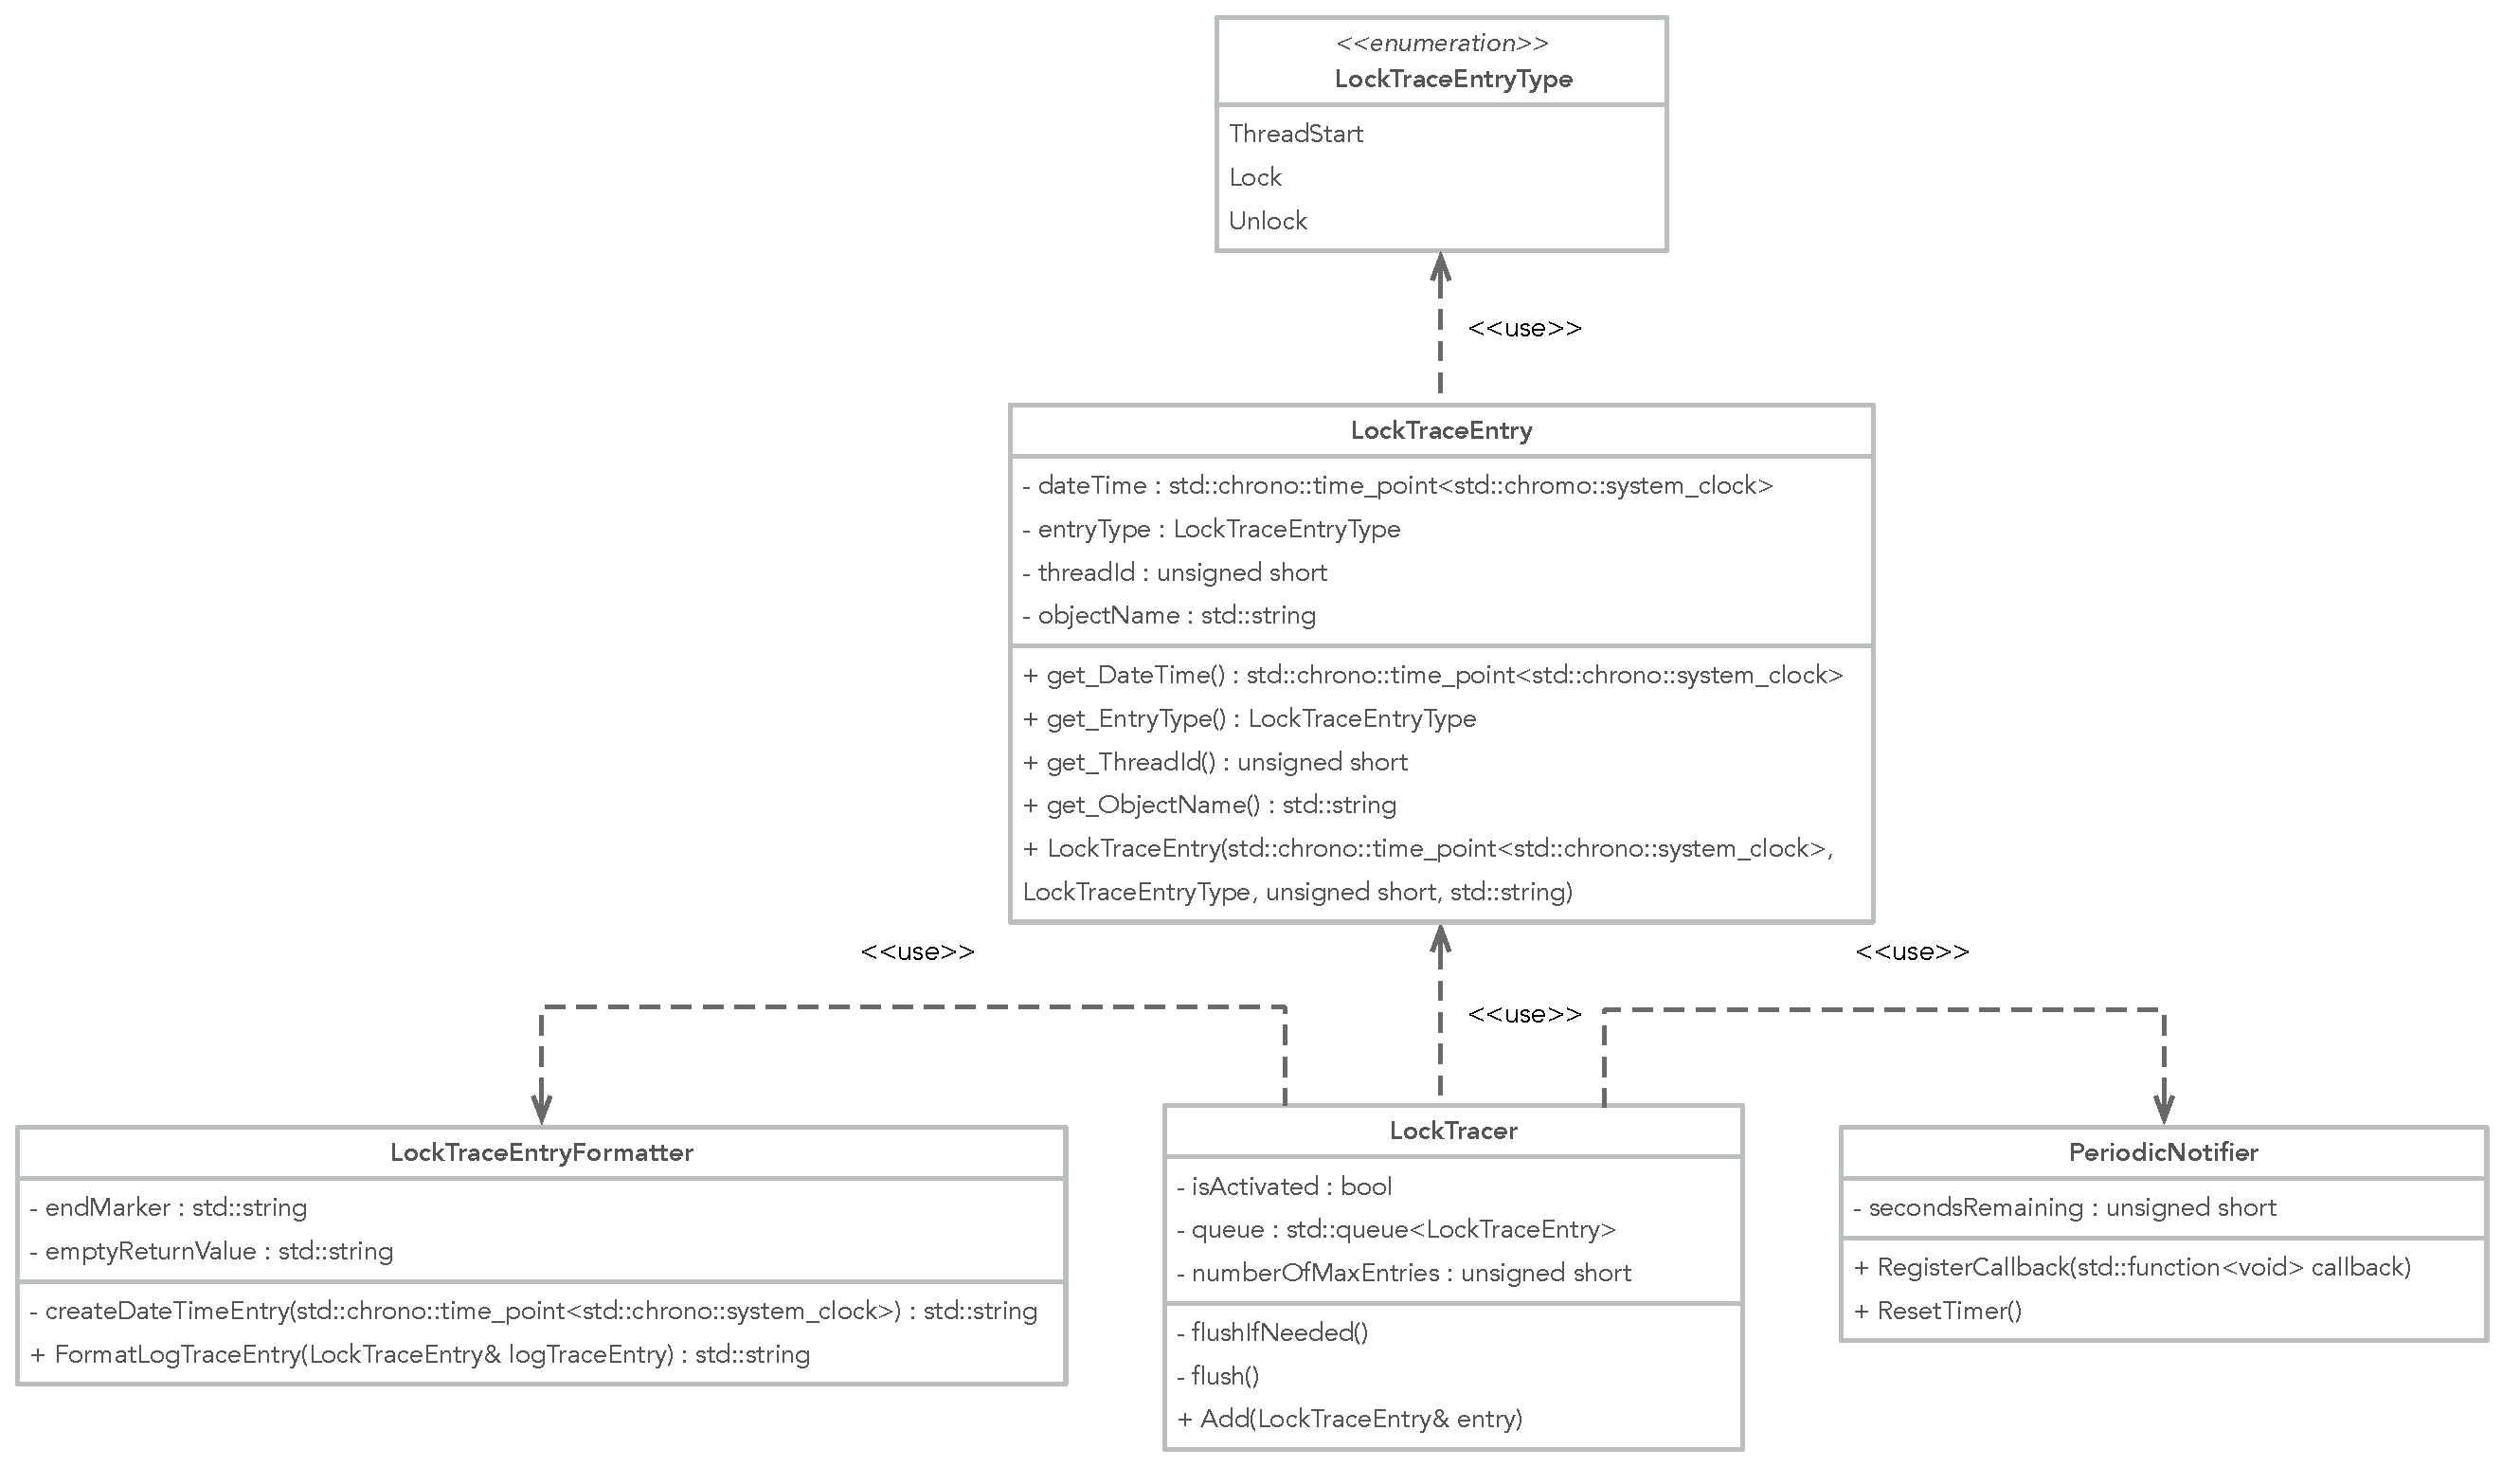
\includegraphics[width=\linewidth]{LockTrace_Design.eps}
  \footnotesize\sffamily Quelle: Eigene Darstellung
  \caption{UML-Klassendiagramm für Trace-Funktionalität}
  \label{fig:LockTrace_Design}
\end{figure}
Die notwendigen Informationen für einen Trace-Eintrag werden in der Klasse
\texttt{Lock\-Trace\-Entry} gehalten. Für den Zeitunkt wird der Typ 
\texttt{chrono::\-time\_point} vom Typ \texttt{chrono::\-high\_\allowbreak resolution\_\allowbreak clock}
verwendet. Der Typ \texttt{chrono::\-high\_\allowbreak resolution\_\allowbreak
clock} stellt einen Zeitpunkt mit der höchstmöglichen Genauigkeit der jeweiligen
Implementierung dar\footnote{C++ ab der Version 11}. Für die spätere
Visualisierung ist eine hohe Genauigkeit notwendig, um nahezu parallel
aufgetretene Lockereignisse chronologisch getrennt visualisieren zu können.

Die Klasse \texttt{Lock\-Trace\-Entry\-Formatter} erstellt mit der Methode
\texttt{Format\-Lock\-Trace\-Entry} aus einem \texttt{Lock\-Trace\-Entry} eine
Zeichenkette, die einer Zeile in der Trace-Datei entspricht. Diese Klasse wird
als Singleton implementiert, da zur Laufzeit immer nur genau eine Instanz
benötigt wird.

Die Klasse \texttt{Lock\-Tracer} stellt die Methode \texttt{Add} zur Verfügung,
welche von der OpenPEARL-Laufzeitumgebung aufgerufen wird. Mit Hilfe der Methode
können Lockereignisse erstellt werden. Die Methode \texttt{IsEnabled} gibt den
aktuellen Zustand der \texttt{Lock\-Tracer}-Instanz zurück. Mithilfe dieser
Methode kann ein Aufrufer prüfen, ob die Trace-Funktionalität aktiviert ist. Ist
dies nicht der Fall, muss die \texttt{Add}-Methode nicht aufgerufen und somit
auch kein \texttt{Lock\-Trace\-Entry}-Objekt erzeugt werden. Die Klasse wird
ebenfalls als Singleton implementiert, damit nur eine Instanz zur Laufzeit
verwendet werden kann.

Das Speichern der Ereignisse in die Trace-Datei ist kostspielig und soll daher
nicht für jeden Eintrag gemacht werden. Die Klasse \texttt{Lock\-Tracer} reiht
dazu die einzelnen Lockereignisse, welche über die \texttt{Add}-Methode
hinzugefügt werden, in eine Warteschlange ein. Sobald eine spezifizierte Anzahl
erreicht ist, wird die Warteschlange geleert und in die Trace-Datei geschrieben.
Die Anzahl kann über die Umgebungsvariable
\texttt{OpenPEARL\_LockTracer\_MaxEntries} spezifiziert werden. Die
Umgebungsvariable wird bei der Initialisierung der
\texttt{Lock\-Tracer}-Implementierung ausgelesen und in der Variable
\texttt{number\-Of\-Max\-Entries} gespeichert.

Das Hinzufügen der Ereignisse in die Warteschlange kann parallel erfolgen und
muss daher threadsicher implementiert werden. Eine Möglichkeit wäre, die
einzelnen Zugriffe über einen Lock zu synchronisieren. Dies würde die Laufzeit
der Anwendung stark negativ beeinflussen. Deswegen wird die lock-freie
Implementierung einer Warteschlange aus \autocite{Moody_Camels_Concurrentqueue}
verwendet. Die Warteschlange garantiert eine threadsichere Implementierung, aber
keine Sortierung innerhalb der Warteschlange für mehrere
Produzenten\footnote{Vgl. "`Reasons not to use"' in
\autocite{Moody_Camels_Concurrentqueue}}. Da es zur Laufzeit nur eine einzige
Instanz der \texttt{Lock\-Tracer}-Klasse gibt, ist die Reihenfolge innerhalb der
Warteschlange dennoch garantiert.

Der Dateipfad zur Speicherung der Trace-Datei wird über die Umgebungsvariable
\texttt{OpenPEARL\_LockTracer\_Path} definiert und bei der Initialisierung der
\texttt{LockTracer}-Implementierung in der Variable \texttt{filePath}
gespeichert.

Die dritte Umgebungsvariable \texttt{OpenPEARL\_LockTracer\_Enabled} wird zur
Aktivierung der Trace-Funktionalität verwendet. Wenn die Umgebungsvariable
gesetzt ist und den Wert \texttt{true} hat, wird die Trace-Funktionalität
aktiviert. Ansonsten werden alle Aufrufe zur \texttt{Add}-Methode direkt über
eine \texttt{return}-Anweisung beendet. Dadurch wird die Laufzeit der Anwendung
bei deaktivierter Trace-Funktionalität nicht beeinflusst.

In der OpenPEARL-Laufzeitumgebung werden die \textrm{REQUEST}- und
\textrm{RELEASE}-Anweisungen in der Semaphor-Implementierung unter
runtime/common/Semaphore.cc implementiert. Bei einer Erhöhung auf eins oder
einer Verringerung auf null eines Semaphors muss ein Lockereignis erzeugt
werden. Bei einer Erhöhung auf eins muss der \texttt{Lock\-Trace\-Entry\-Type}
\texttt{Unlock} bei einer Verringerung auf null der
\texttt{Lock\-Trace\-Entry\-Type} \texttt{Lock} verwendet werden. Die Klassen
für die Implementierung des LockTracers müssen bei der Kompilierung der
OpenPEARL-Laufzeitumgebung mit einbezogen werden. In der Datei
runtime/common/Files.common sind alle Dateien aufgeführt, welche bei der
Kompilierung einbezogen werden. Dort müssen die Dateien, die aus
\cref{fig:LockTrace_Design} entstehen eingetragen werden.

\section{Analysieren der Trace-Datei}
\label{section:Analysieren der Trace-Datei}
Als Eingabe dient die in \cref{section:Erzeugung der Trace-Datei} erzeugte
Trace-Datei. Die Trace-Datei wird Zeile für Zeile ausgelesen. Die einzelnen
Lockereignisse werden nach den jeweiligen Threads gruppiert. Anschließend wird
ein zweidimensionaler Graph erzeugt.

Jede Thread-Gruppe bildet einen horizontalen Strahl ab, auf dem die zugehörigen
Lockereignisse dargestellt werden. Für die Darstellung der einzelnen Zeitpunkte
werden nur die jeweiligen Deltas zum frühesten Zeitpunkt verwendet. Die Abszisse
startet demnach mit dem Wert null, der dem frühesten Zeitpunkt entspricht. Eine
mögliche Darstellung ist in \cref{fig:Timeline_Example} skizziert.
\begin{figure}[ht]
  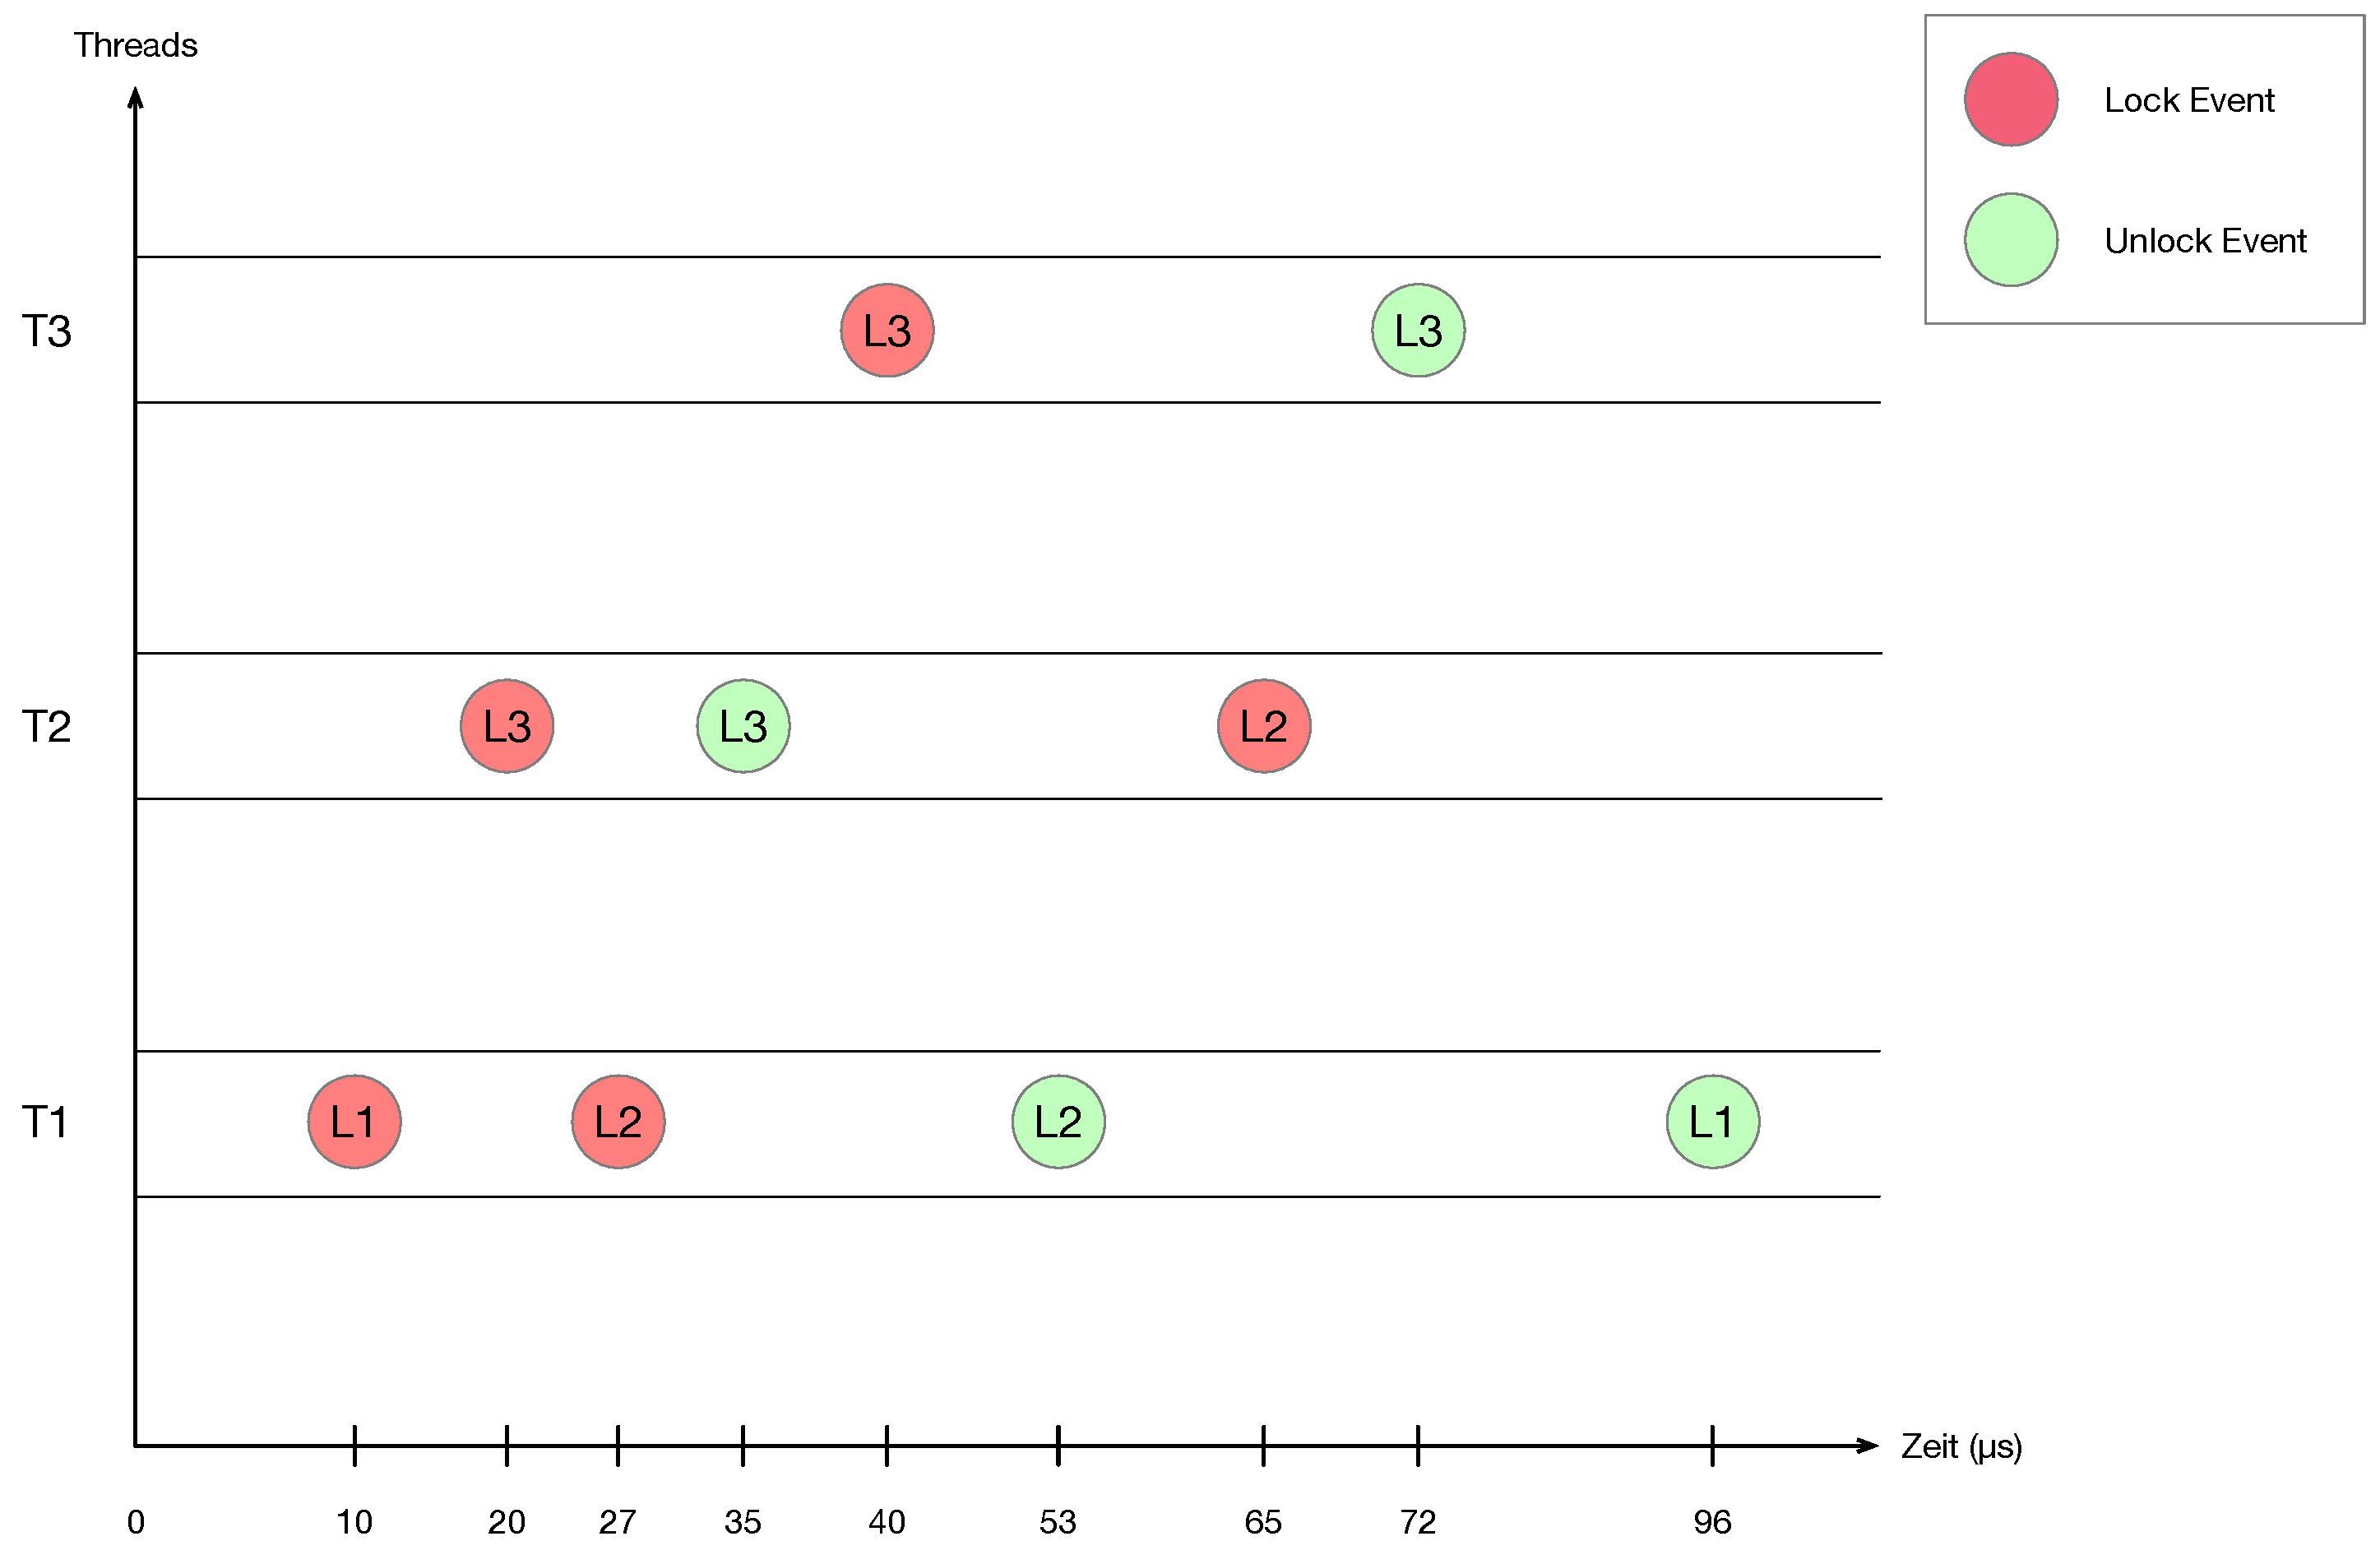
\includegraphics[width=\linewidth]{Timeline_Example.eps}
  \caption{Visualisierung der chronologischen Verwendung von \textrm{SEMA}-Objekten}
  \label{fig:Timeline_Example}
\end{figure}

\section{Erweiterung: Potenzielle Deadlocks}
\label{section:Erweiterung: Potenzielle Deadlocks}
Als Eingabe dient wieder die Trace-Datei aus \cref{section:Erzeugung der
Trace-Datei}. Die Lockereignisse werden Zeile für Zeile aus der Trace-Datei
ausgelesen und in einen \emph{execution trace} überführt\footnote{Siehe
\cref{section:Deadlockerkennung allgemein}}. Dieser wird als Eingabe für den
Algorithmus aus \cref{section:MagicLock} verwendet. Der Algorithmus liefert
einen Lockgraphen mit potenziellen Deadlocks, welche als Zyklen im Graphen zu
erkennen sind, zurück. Der Lockgraph wird dem Anwender, wie in
\cref{fig:Magiclock_Example} skizziert, dargestellt.
\begin{figure}[ht]
  \begin{center}
    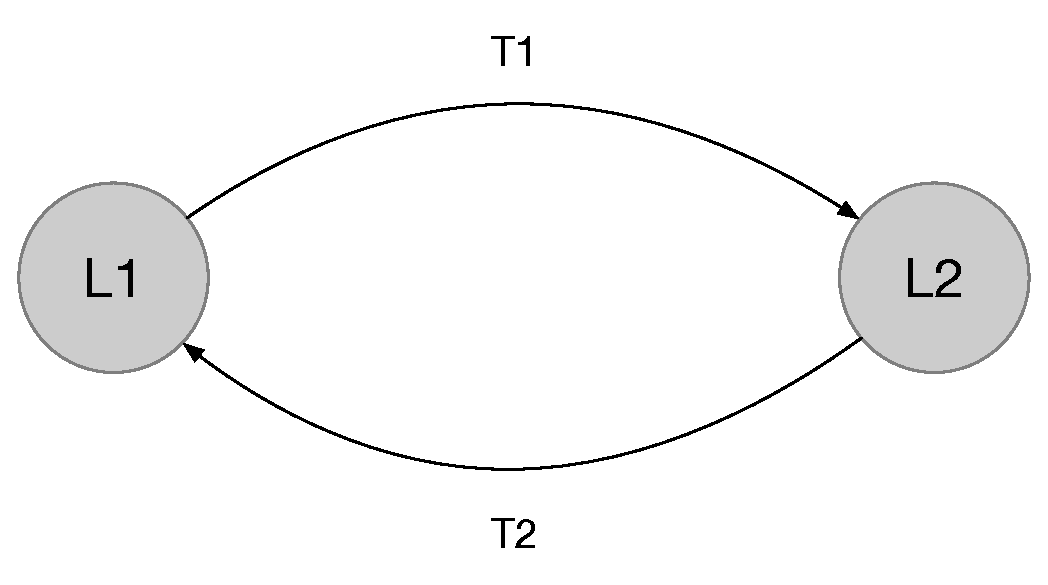
\includegraphics[width=\linewidth/2]{Magiclock_Example.eps}
  \end{center}
  \footnotesize\sffamily Quelle: Eigene Darstellung
  \caption{Visualisierung eines potentiellen Deadlocks}
  \label{fig:Magiclock_Example}
\end{figure}